% ============================================================
% Betting on War: Prediction Markets, Anonymous Costly Signals,
% and Strategic Deception in International Crises
%
% Target: American Political Science Review (APSR)
% ============================================================
\documentclass[12pt]{article}

% ---------- Packages ----------
\usepackage[margin=1in]{geometry}
\usepackage{setspace}
\doublespacing
\usepackage{amsmath,amssymb,amsthm}
\usepackage{mathtools}
\usepackage{graphicx}
\usepackage[hidelinks]{hyperref}
\usepackage{natbib}
\bibliographystyle{apsr}
\usepackage{booktabs}
\usepackage{caption}
\usepackage{subcaption}
\usepackage{float}
\usepackage{tikz}
\usetikzlibrary{arrows.meta, positioning, calc}
\usepackage{enumitem}
\usepackage{url}
\usepackage{xcolor}
\usepackage{thmtools}

% ---------- Theorem Environments ----------
\newtheorem{proposition}{Proposition}
\newtheorem{corollary}{Corollary}
\newtheorem{lemma}{Lemma}
\newtheorem{definition}{Definition}
\newtheorem{remark}{Remark}
\newtheorem{hypothesis}{Hypothesis}

% ---------- Custom Commands ----------
\newcommand{\E}{\mathbb{E}}
\newcommand{\Pr}{\text{Pr}}
\newcommand{\R}{\mathbb{R}}

% ============================================================
\begin{document}

\title{Betting on War: Prediction Markets, Anonymous Costly Signals, and Strategic Deception in International Crises}

\author{%
Jonathan Walberg\\
\textit{University of Virginia}\\
\texttt{jdw5vq@virginia.edu}
}

\date{\today}

\maketitle

\begin{abstract}
How do prediction markets alter signaling dynamics in international crises, and under what conditions can states exploit them to generate credible signals of resolve? This paper introduces the concept of \textit{anonymous costly signals}---a new category in crisis bargaining theory. Unlike traditional costly signals (mobilizations, public threats, alliance commitments), prediction market bets are (1) costly, imposing real financial exposure; (2) public, producing observable probability shifts; (3) anonymous, concealing the sender's identity; and (4) plausibly informational, interpreted as insider knowledge rather than deliberate signaling. I develop a formal signaling game in which the sender chooses an anonymous market position, the market produces a public signal, and the receiver updates beliefs through a deception-channel parameter $\lambda$ capturing the probability that the observed order flow reflects a leak versus strategic manipulation. A separating equilibrium exists in which resolved types place large bets and unresolved types do not. Higher ``leak plausibility'' ($\lambda$) lowers signaling costs, and a haversack ruse extension shows how false bets can generate tactical deception. I test the theory's predictions using original data from Polymarket and Kalshi on geopolitical contracts, finding that crisis events systematically move prediction market prices, that market shocks sometimes precede public events, and that effects are concentrated in thin markets---consistent with the mechanism of anonymous costly signaling.

\vspace{0.5em}
\noindent\textbf{Keywords:} crisis bargaining, costly signaling, prediction markets, strategic deception, anonymous signals, information aggregation
\end{abstract}

\newpage
\tableofcontents
\newpage

% ============================================================
% SECTION 1: INTRODUCTION
% ============================================================
\section{Introduction}

Prediction markets are increasingly treated as real-time indicators of geopolitical risk. Contracts on whether Israel will strike Iran, whether the United States will intervene in a regional war, or whether China will move militarily against Taiwan generate continuously updated prices that are read by journalists, analysts, investors, and policymakers as estimates of what informed observers think will happen. In ordinary usage, these markets are treated as forecasting devices. In international crises, however, they may do more than aggregate expectations. They may become part of the signaling environment itself.

This article argues that prediction markets introduce a new mechanism into crisis bargaining: \textit{anonymous costly signals}. Unlike traditional signals of resolve, such as troop mobilizations, public threats, or alliance commitments, prediction-market signals impose real costs while concealing the sender's identity. A large market move can therefore appear to reflect insider information rather than intentional communication. That ambiguity matters. Because observers often treat prediction-market prices as evidence of dispersed knowledge or privileged access, a state or state-aligned actor may be able to generate a credible-looking signal of hidden intent at a fraction of the cost of conventional military signaling.

The claim is not merely that markets can be manipulated, nor only that insider trading is possible. It is that even in a world of stronger enforcement and cleaner market rules, geopolitical prediction markets would still alter crisis dynamics because their prices can be interpreted as meaningful evidence about private intentions. In that sense, these markets do not simply forecast crises from the outside. They can shape how states interpret one another during crises, making them relevant to bargaining, deterrence, and strategic deception.

Recent events have made this argument uncomfortably concrete. In March 2026, CNN reported that a single trader had earned nearly \$1 million on Polymarket through dozens of well-timed bets that correctly predicted U.S. and Israeli military operations against Iran, winning 93\% of five-figure wagers on unannounced military operations. Israeli authorities indicted a military reservist and a civilian for allegedly using classified briefing information to place bets on Polymarket ahead of the June 2025 strikes on Iranian nuclear facilities, earning \$162,663 from a single wager placed the day before operations began. Another account, trading as ``Magamyman,'' made \$553,000 on bets tied to the death of Iran's Supreme Leader just hours before strikes occurred. These are not hypothetical scenarios. They are the mechanism this paper theorizes, observed in real time.

The paper proceeds as follows. Section~\ref{sec:lit} situates the argument within three literatures: crisis bargaining and costly signaling, strategic deception, and the political economy of prediction markets. Section~\ref{sec:theory} develops the theoretical argument for anonymous costly signals. Section~\ref{sec:model} presents a formal signaling game with complete proofs and equilibrium characterization. Section~\ref{sec:empirical} describes the empirical strategy and presents results from an event study using original prediction market data. Section~\ref{sec:experiment} outlines a survey experiment design for future testing. Section~\ref{sec:implications} discusses implications for deterrence, crisis stability, and information warfare. Section~\ref{sec:conclusion} concludes.


% ============================================================
% SECTION 2: LITERATURE REVIEW
% ============================================================
\section{Literature Review}\label{sec:lit}

The argument sits at the intersection of three literatures: crisis bargaining and costly signaling, strategic deception, and the political economy of prediction markets. Each contributes essential elements; none, on its own, captures the mechanism this paper identifies.

\subsection{Crisis Bargaining and Costly Signaling}

The starting point is the rationalist bargaining literature on war, especially the claim that conflict is puzzling because war is costly and therefore there should usually exist negotiated settlements that both sides prefer to fighting. In \citet{fearon1995}'s formulation, the puzzle is not simply why states disagree, but why they fail to locate bargains that would leave both sides better off than war. His answer centers on two mechanisms: private information with incentives to misrepresent, and commitment problems. For this paper, the first mechanism matters most. States possess private information about capabilities, resolve, and the value they attach to the issue at stake, and because they want favorable bargaining outcomes, they cannot simply reveal that information credibly through cheap talk.

That move in the literature is what makes signaling central to crisis bargaining. Once one assumes that states cannot credibly announce their type, the next question is how they can communicate resolve in ways that receivers will believe. The costly signaling literature answers by showing that actions can reveal private information when they are differentially bearable across types \citep{spence1973, fearon1997}. \citet{kydd2005}'s reassurance model makes this logic explicit: signals work not because they are dramatic, but because they impose risks that resolved types are more willing to bear than unresolved types.

\citet{fearon1997}'s distinction between tying hands and sinking costs has become especially influential. Leaders can tie hands by creating domestic or reputational penalties if they back down, or they can incur sunk costs by mobilizing forces or otherwise paying resources in advance to demonstrate seriousness \citep{yarhimilokertzer2018}. In both cases, the sender openly takes an action that audiences and adversaries can observe and interpret as reflecting willingness to bear consequences. \citet{quek2021} extends this framework by identifying four distinct costly signaling mechanisms, while \citet{kertzerrathbun2019} show that the credibility of signals depends not only on their costliness but on how recipients process them---a point that becomes especially relevant when signals are anonymous.

The common feature across this literature is that credibility is attached to \textit{attributable acts}. States mobilize. Leaders threaten publicly. Governments make commitments that can later be judged. The literature generally presumes that receivers may be uncertain about whether the sender is sincere, but not about \textit{who is sending the message}. Prediction markets complicate that structure fundamentally.

\subsection{Endogenous Uncertainty and Information Environments}

A second important branch asks where the uncertainty that drives crisis bargaining originates. \citet{meirowitzandsartori2008} show that states may actively \textit{create} the uncertainty that later destabilizes bargaining. In their account, states can begin with complete information and nonetheless choose strategies of military acquisition and secrecy that leave adversaries uncertain about exact levels of capability. Their argument broadens the rationalist tradition by demonstrating that the informational environment of bargaining is itself strategically produced. States do not merely conceal information once bargaining begins; they shape the conditions under which relevant information can be known at all.

This insight matters directly for the present argument. If states can shape the informational systems through which others infer hidden intent, then prediction markets represent a new medium through which such shaping can occur. Related work by \citet{debsmonteiro2014} reinforces the broader lesson: many of the conditions that destabilize bargaining are produced by strategic choice. States invest, conceal, and posture in ways that alter what rivals know and fear.

\subsection{Strategic Deception}

A third relevant literature concerns strategic deception and the manipulation of information environments. \citet{jervis1970, jervis1976} underscores how states try to manipulate the variables that shape others' expectations, distinguishing between ``signals'' (actions taken specifically to communicate) and ``indices'' (actions that are informative because they are costly to fake). \citet{mearsheimer2011} catalogs the varieties of state lying in international politics. \citet{trager2017} examines how diplomatic communication can convey meaningful information despite incentives to misrepresent. \citet{yarhimilo2014} shows how intelligence services attempt to read adversary intentions through observable indicators.

This literature is rich on deception through overt communication, intelligence, and military behavior, but notably thin on deception through \textit{financial information systems}. Existing work helps explain why states seek to influence what others believe and why ambiguity can be strategically valuable. What it does not yet provide is a theory of how market-based signals---especially signals that are public, costly, and anonymous---fit into that broader ecology of deception.

\subsection{Prediction Markets and Information Aggregation}

The final body of relevant work comes from the political economy of information markets. The core assumption is that market prices aggregate dispersed information and therefore provide socially useful estimates about uncertain future events \citep{wolferszitzewitz2004, arrow2008}. \citet{tetlock2005} and \citet{tetlockgardner2015} document how prediction markets and structured forecasting can outperform expert judgment.

\citet{hanson2009} argues, provocatively, that a manipulator can actually \textit{aid} prediction market accuracy by providing liquidity and incentivizing informed counter-trading. Experimental evidence has been more mixed: \citet{hanson2006} find that manipulators in laboratory markets are unable to persistently distort prices, while \citet{dekkerseidl2023} show that mere \textit{suspicion} of manipulation erodes trust in market signals and leads to suboptimal policy decisions. Recent large-scale field experiments find that manipulation effects persist for up to 60 days, though they fade over time and are harder to sustain in thick markets \citep{manipulability2025}.

The gap across these literatures is specific. The crisis bargaining literature assumes credible signals are attributable acts. The deception literature examines perception manipulation through diplomacy, intelligence, and military posture. The prediction market literature treats prices as informational outputs rather than strategic inputs. Missing is an account of how actors can use anonymous financial exposure to generate public signals that look less like overt coercion than like information leakage. That is the opening for this paper.


% ============================================================
% SECTION 3: THEORY OF ANONYMOUS COSTLY SIGNALS
% ============================================================
\section{Theory: Anonymous Costly Signals in Crisis Bargaining}\label{sec:theory}

\subsection{Costly Signaling and the Problem of Believable Intent}

Crisis bargaining is difficult for a familiar reason: states often possess private information about capabilities, resolve, and willingness to fight, and they have incentives to misrepresent that information when bargaining over the status quo. The costly signaling literature responds by showing that actions can reveal private information when they are differentially bearable across types. The signal is believable not because it is dramatic, but because it is differentially costly.

Yet existing signaling logics generally presume that signals are \textit{attributable}. Someone mobilizes. Someone threatens. Someone deploys. Prediction markets complicate that structure. They produce publicly visible movements in assessed probabilities, but not publicly visible senders. What becomes observable is not a mobilization, a statement, or a deployment, but a shift in the market's implied expectation that a particular event will occur. The result is a signal that is public, costly, and consequential, yet \textit{unattributed}. That combination creates a qualitatively different signaling environment.

\subsection{Prediction Markets as Strategic Objects}

Prediction markets are commonly understood as information aggregators. Their appeal lies precisely in the belief that they synthesize dispersed information into a single publicly interpretable price. In geopolitical settings, however, the same reputation can make them strategically vulnerable. If observers believe that a large price movement probably reflects crowd wisdom, privileged information, or some diffuse aggregation of informed judgment, then a well-timed market move can do more than register beliefs. It can manufacture them.

The argument is not that all market movements are manipulative, nor that observers are irrational. It is instead that the \textit{social meaning} of market prices changes the strategic environment. Prediction markets are read as if they contain information. That belief need not be wrong in general for it to be exploitable in specific cases. A state, intelligence service, aligned financier, or proxy actor does not need everyone to think a market price is certain proof of hidden intent. It needs only enough relevant observers to treat a sudden spike as evidence that someone, somewhere, knows something. Once that inference becomes plausible, the market no longer functions solely as an external measure of expectations. It becomes part of the crisis itself.

This helps explain why prediction-market signaling is distinct from propaganda or overt disinformation. Propaganda is often discounted because its source is visible and its strategic intent is obvious. A market spike is processed differently. The source is obscured. The cost is real. The movement appears to emerge from a system supposedly designed to aggregate information rather than broadcast intentions. The receiver is therefore not merely asking whether the sender is lying. The receiver is asking what hidden information the market may be revealing. That is a very different inferential problem, and it is one that may be more advantageous to a sophisticated deceiver.

\subsection{The Concept: Anonymous Costly Signals}

\begin{definition}[Anonymous Costly Signal]
An \textit{anonymous costly signal} is a publicly observable action that (i) imposes real costs on the sender, (ii) conceals the sender's identity, and (iii) is plausibly interpreted by receivers as revealing insider information rather than deliberate strategic communication.
\end{definition}

Prediction-market trades fit this definition especially well. A sufficiently large purchase of contracts tied to a military strike can move prices sharply. That move is observable to all market participants and often to a much wider public once it is reported or amplified. The trader incurs real financial exposure, so the act is not costless. But because the identity behind the trade is concealed, observers cannot easily distinguish among several plausible interpretations: genuine insider trading, informed speculation, distributed private knowledge, or strategic manipulation. The signal's persuasive force comes from that ambiguity, not despite it.

This is the mechanism's core novelty. In standard signaling stories, credibility usually comes from the sender openly bearing a cost. Here, cost still matters, but attribution recedes. The receiver observes the costly trace without securely identifying the actor who produced it. Instead of asking whether a known sender has taken a costly action to demonstrate resolve, the receiver asks whether an observed market movement is more likely to have been generated by true private knowledge or by strategic intervention. A signal that looks like a \textit{leak} can be more persuasive than a signal that looks like a \textit{warning}. Leaks imply hidden reality. Warnings imply strategic intent.

\subsection{Why Anonymity Can Increase Credibility}

At first glance, anonymity should weaken signaling: if the receiver cannot identify the sender, why treat the signal as informative? The answer is that anonymity changes the \textit{source} of meaning. Traditional signals derive credibility from visible authorship and visible cost. Anonymous costly signals derive credibility from visible \textit{effect} and \textit{uncertain origin}. The receiver does not need to identify the exact trader to infer that the market movement may be connected to private information inside the sender's political or military apparatus.

Crises are environments of asymmetric information and high consequence. Receivers often respond not to certainty but to plausible worst-case interpretation. A move need not be definitively attributable to a state for it to matter strategically. It need only raise the posterior probability that informed actors expect escalation. Moreover, the more prediction markets gain public legitimacy as forecasting tools, the more difficult it becomes for decision-makers to dismiss large moves as irrelevant noise. Prediction markets borrow their strategic power from their reputation as epistemic institutions.

Anonymity may even make the signal \textit{more} persuasive than an overt message for a second reason: plausible deniability. If a state publicly threatens attack, the receiver discounts the message because the sender clearly wants the receiver to update in a particular direction. If a market suddenly moves, the same receiver may suspect that someone with privileged information has acted on it rather than trying to persuade. The signal therefore appears less like communication and more like revelation.

\subsection{Why States Would Use This Channel}

If traditional signaling tools already exist, why would states bother with market manipulation? The most direct answer is cost. Military signals can be expensive, slow, escalatory, and politically constraining. Moving forces, changing deployments, or issuing public threats can create diplomatic backlash, reveal operational information, or commit leaders to courses of action they may later regret. Prediction-market signals, by contrast, can be cheap, fast, deniable, and scalable. A relatively modest financial outlay in a thin market may generate a visible probability shift large enough to affect observers' beliefs.

The point is not that market signaling will replace conventional signaling. Rather, prediction markets offer a \textit{supplementary channel} that is especially attractive when a state wants to shift adversary expectations without openly escalating, when it wants to test reactions before acting, or when it wants to preserve deniability while still shaping the informational environment.

The same logic explains why proxies matter. Governments need not trade directly. The ideal manipulator is a proxy sufficiently connected to act with purpose but sufficiently distant to preserve uncertainty about source. That uncertainty is not a flaw in the mechanism. It is one of the mechanism's conditions of success.

\subsection{The Receiver's Inference Problem}

The receiver observes a market movement but does not observe the motive or identity behind it. It must choose among at least three interpretations: (1) real private information held by actors with genuine knowledge; (2) ordinary information aggregation among traders reacting to public and semi-public signals; and (3) strategic manipulation intended to create precisely the inference that the first interpretation implies. In crises, these possibilities collapse into one another because the same observable market move is consistent with all three.

This mixture is what gives anonymous costly signals their strategic value. If receivers could perfectly separate genuine insider information from deliberate manipulation, the mechanism would weaken dramatically. But they generally cannot. The receiver therefore updates under \textit{uncertainty about uncertainty}: it is not simply revising beliefs about whether the sender is resolved, but revising beliefs about whether the market contains hidden evidence about the sender's resolve.

\subsection{Two Mechanisms: Signaling and the Haversack Ruse}

The theory identifies two distinct strategic uses of prediction markets in crises:

\begin{enumerate}[label=\textbf{\arabic*.}]
    \item \textbf{Credibility enhancement through costly market signals.} A state places bets consistent with its true intentions, using the market to generate a credible public signal that increases the probability of the adversary conceding. The market position is costly and sincere---the sender \textit{does} intend to strike---but the signal reaches the adversary through an anonymous financial channel rather than through official communication. This is the mechanism that brings the adversary to the bargaining table.

    \item \textbf{Tactical deception through false bets (the haversack ruse).} A state places bets that are \textit{inconsistent} with its true intentions to mislead about timing, location, or target. ``Bet Friday, bomb Thursday.'' ``Bet here, strike there.'' The financial exposure is real but modest compared to the tactical advantage of misdirection. This extends the classical military deception tradition---from Operation Mincemeat to the Haversack Ruse of 1917---into the domain of financial information systems.
\end{enumerate}

\subsection{Scope Conditions}

The mechanism should not be expected to operate uniformly. Anonymous costly signals should be most potent under several conditions:
\begin{itemize}
    \item The market is \textit{thin} enough that moderate trades can move price.
    \item The platform is \textit{visible} enough that relevant audiences will notice.
    \item The issue is \textit{salient} enough that observers are primed to infer hidden information.
    \item Public information is \textit{incomplete} enough that a sudden market move seems especially diagnostic.
\end{itemize}

By contrast, the mechanism should weaken in thick markets where manipulation is expensive, in obscure markets no policymaker watches, or in cases where public evidence already makes the outcome obvious. These scope conditions help explain why the mechanism depends on a fairly modern institutional environment: it requires liquid-enough geopolitical contracts, widespread interpretive attention to market prices, and an audience accustomed to reading prediction markets as informative.


% ============================================================
% SECTION 4: FORMAL MODEL
% ============================================================
\section{Formal Model}\label{sec:model}

This section develops a signaling game that formalizes the mechanism of anonymous costly signals. The model builds explicitly on \citet{fearon1997}'s sunk-cost signaling framework but introduces two novel features: the signal is anonymous, and the receiver's belief updating incorporates a deception-channel parameter $\lambda$ that captures the probability the observed market movement reflects insider information rather than strategic manipulation.

\subsection{Players, Types, and Timing}

\textbf{Players.} There are two players: a Sender $S$ (e.g., Israel/U.S. decision-making coalition) and a Receiver $R$ (e.g., Iran).

\textbf{Types.} Nature draws $S$'s private type $\theta \in \{H, L\}$ with prior probability $\Pr(\theta = H) = p_0$. Type $H$ (``high resolve'') is willing to carry out a military strike if challenged. Type $L$ (``low resolve'') prefers to avoid striking.

\textbf{Timing.}
\begin{enumerate}
    \item Nature draws $\theta$, observed by $S$ but not $R$.
    \item $S$ chooses an anonymous market position $\beta \geq 0$ in a prediction market contract paying 1 if ``strike occurs'' by a deadline, 0 otherwise.
    \item The market produces a public signal $m = \beta + \varepsilon$, where $\varepsilon \sim F_\varepsilon$ is noise from other traders, with density $f_\varepsilon$ symmetric and continuous around zero.
    \item $R$ observes $m$ but not the identity of the trader. $R$ also believes that with probability $\lambda \in [0,1)$, the observed order flow was generated by an informed insider (a ``leak'') rather than by $S$'s strategic manipulation.
    \item $R$ chooses action $a_R \in \{\text{Concede}, \text{Resist}\}$.
    \item If $R$ resists, $S$ chooses action $a_S \in \{\text{Strike}, \text{No Strike}\}$.
\end{enumerate}

This mirrors \citet{fearon1997}'s crisis sequence---signal, response, follow-through---except the signal is an anonymous sunk cost embedded in a market rather than a troop mobilization.

\subsection{Information Structure: The Deception Channel}

The key innovation is the parameter $\lambda$, which captures the receiver's belief about the source of market movements. Formally, $R$ believes:
\begin{itemize}
    \item With probability $(1-\lambda)$: the order flow was generated by $S$ (strategic manipulation).
    \item With probability $\lambda$: the order flow was generated by an informed insider whose trading activity is correlated with the true state of the world (an apparent ``leak'').
\end{itemize}

Under the leak interpretation, let $g_H(m)$ denote the density of market signals generated by informed traders when a strike is truly likely ($\theta = H$), and let $g_L(m)$ denote the density when it is not ($\theta = L$). We assume a monotone likelihood ratio property: $g_H(m)/g_L(m)$ is increasing in $m$.

$R$'s posterior belief that $\theta = H$ given observed market signal $m$ is:
\begin{equation}\label{eq:posterior}
\mu(m) \equiv \Pr(\theta = H \mid m) = \frac{p_0 \left[(1-\lambda) f_\varepsilon(m - \beta_H) + \lambda g_H(m)\right]}{p_0 \left[(1-\lambda) f_\varepsilon(m - \beta_H) + \lambda g_H(m)\right] + (1-p_0)\left[(1-\lambda) f_\varepsilon(m - \beta_L) + \lambda g_L(m)\right]}
\end{equation}

This is the formal encoding of the receiver's attributional uncertainty: the receiver cannot tell if a big market move is a deliberate signal or information revelation via a leak.

\subsection{Payoffs}

\textbf{Receiver payoffs.} If $R$ concedes, it pays concession cost $c > 0$ but avoids strike damage:
\begin{equation}
u_R(\text{Concede}) = -c
\end{equation}
If $R$ resists and $S$ strikes, $R$ suffers damage $d > c$:
\begin{equation}
u_R(\text{Resist}, \text{Strike}) = -d
\end{equation}
If $R$ resists and $S$ does not strike:
\begin{equation}
u_R(\text{Resist}, \text{No Strike}) = 0
\end{equation}

$R$ concedes if and only if its posterior probability of a strike exceeds the threshold:
\begin{equation}\label{eq:threshold}
\mu^* \equiv \frac{c}{d}
\end{equation}

\textbf{Sender payoffs.} Let $B > 0$ denote the benefit to $S$ if $R$ concedes, $k > 0$ the cost of striking, and $\phi > 0$ the per-unit cost of market position. The sender's payoffs, incorporating market exposure, are:

\begin{align}
u_S(\text{Concede}; \beta) &= B - \phi\beta \label{eq:s_concede}\\
u_S(\text{Resist}, \text{Strike}; \beta) &= B - k + \beta - \phi\beta \label{eq:s_strike}\\
u_S(\text{Resist}, \text{No Strike}; \beta) &= -\phi\beta \label{eq:s_nostrike}
\end{align}

The term $\beta - \phi\beta$ in (\ref{eq:s_strike}) captures the fact that if the strike occurs, the prediction market contract pays out, partially offsetting costs. If no strike occurs, the position loses $\phi\beta$.

\textbf{Type restriction.} We impose that $H$-types prefer to strike after resistance ($B - k > 0$) while $L$-types prefer not to ($B - k < 0$, or equivalently, $L$-types face higher effective $k$). This replicates Fearon's resolved vs.\ unresolved distinction.

\subsection{Strategies and Equilibrium Concept}

A strategy for $S$ is a mapping $\sigma_S: \{H, L\} \to \R_+$ choosing bet size $\beta$. A strategy for $R$ is $\sigma_R: \R \to \{\text{Concede}, \text{Resist}\}$. We look for Perfect Bayesian Equilibrium (PBE).

\subsection{Separating Equilibrium}

\begin{proposition}[Existence of Separating Equilibrium]\label{prop:sep}
Under standard regularity conditions on $f_\varepsilon$ and parameter values such that type $H$ prefers Strike and type $L$ prefers No Strike after resistance, there exists a bet size $\beta^* > 0$ and a signal cutoff $\bar{m}$ such that:
\begin{equation}
\sigma_S^*(\theta) = \begin{cases} \beta^* & \text{if } \theta = H \\ 0 & \text{if } \theta = L \end{cases}
\end{equation}
and $R$ concedes if and only if $m \geq \bar{m}$, constituting a PBE.
\end{proposition}

\begin{proof}
Given the candidate strategies, $R$'s concession rule is a cutoff $\bar{m}$ such that $\mu(\bar{m}) = \mu^* = c/d$.

\textbf{Incentive compatibility for type $H$.} Type $H$ chooses $\beta^*$ over $\beta = 0$. Let $\pi_H(\beta)$ denote the probability that $R$ concedes when $H$ chooses $\beta$:
\begin{equation}
\pi_H(\beta) = \Pr(m \geq \bar{m} \mid \beta) = 1 - F_\varepsilon(\bar{m} - \beta)
\end{equation}

$H$'s expected payoff from $\beta^*$:
\begin{equation}
V_H(\beta^*) = \pi_H(\beta^*)(B - \phi\beta^*) + (1 - \pi_H(\beta^*))(B - k + \beta^* - \phi\beta^*)
\end{equation}

$H$'s expected payoff from deviating to $\beta = 0$:
\begin{equation}
V_H(0) = \pi_H(0) \cdot B + (1 - \pi_H(0))(B - k)
\end{equation}

Incentive compatibility requires $V_H(\beta^*) \geq V_H(0)$.

\textbf{Incentive compatibility for type $L$.} Type $L$ chooses $\beta = 0$ over $\beta^*$. If $L$ deviates to $\beta^*$ and $R$ resists, $L$ chooses No Strike, yielding payoff $-\phi\beta^*$.

$L$'s expected payoff from $\beta = 0$:
\begin{equation}
V_L(0) = \pi_L(0) \cdot B + (1 - \pi_L(0)) \cdot 0 = \pi_L(0) B
\end{equation}

$L$'s expected payoff from deviating to $\beta^*$:
\begin{equation}
V_L(\beta^*) = \pi_L(\beta^*)(B - \phi\beta^*) + (1 - \pi_L(\beta^*))(-\phi\beta^*)
\end{equation}

Incentive compatibility requires $V_L(0) \geq V_L(\beta^*)$.

Combining, there exists $\beta^*$ satisfying both constraints when $B - k > 0$ for $H$ and $\phi$ is sufficiently large that $L$ cannot profitably mimic. The separating cost structure is exactly the Spence/Fearon logic: the market exposure functions as a sunk cost that is more bearable for resolved types because they expect to profit from the contract payout.

For off-equilibrium beliefs, we apply the Cho-Kreps intuitive criterion: for any $m$ below $\bar{m}$, $R$ assigns $\mu = 0$ (since only $L$ would benefit from a lower bet), supporting the equilibrium.
\end{proof}

\subsection{The Role of Leak Plausibility}

\begin{proposition}[Leak Plausibility Lowers Signaling Costs]\label{prop:lambda}
Holding fixed the receiver's concession threshold $\mu^*$, an increase in $\lambda$ weakly decreases the minimal bet size $\beta^*$ required for type $H$ to induce concession in equilibrium.
\end{proposition}

\begin{proof}
When $\lambda > 0$, the receiver's posterior $\mu(m)$ from equation~(\ref{eq:posterior}) incorporates the leak-driven likelihood $g_H(m)$. By the monotone likelihood ratio property of $g_H/g_L$, large values of $m$ are more likely under the leak hypothesis when $\theta = H$. This inflates $\mu(m)$ for any given $m$ beyond what the strategic-manipulation channel alone would produce.

Formally, let $\mu_0(m)$ denote the posterior when $\lambda = 0$ and $\mu_\lambda(m)$ the posterior when $\lambda > 0$. For $m$ in the relevant range:
\begin{equation}
\mu_\lambda(m) \geq \mu_0(m) \quad \text{whenever } \frac{g_H(m)}{g_L(m)} \geq \frac{f_\varepsilon(m - \beta_H)}{f_\varepsilon(m - \beta_L)}
\end{equation}

Since $\mu_\lambda(\bar{m}) = \mu^*$ defines the cutoff, and $\mu_\lambda$ is increasing in $\lambda$ for fixed $m$ in the relevant region, the cutoff $\bar{m}$ decreases with $\lambda$. A lower $\bar{m}$ means a smaller $\beta^*$ suffices for $H$ to achieve $\pi_H(\beta^*) \geq \pi_H^{\min}$.
\end{proof}

\begin{remark}
This is the deception result. The state does not need to create a fully transparent costly signal; it can create an ambiguous signal that the receiver may interpret as independent information revelation. Higher $\lambda$ effectively ``subsidizes'' the signal's credibility by borrowing from the market's epistemic reputation.
\end{remark}

\subsection{Shadow of the Future and Reputational Stakes}

To connect to coercive bargaining theory \citep{sechser2018}, we extend the model by letting the receiver's concession cost include a reputational component:
\begin{equation}
c(\delta) = c_0 + \delta \cdot r
\end{equation}
where $c_0$ is the immediate policy concession cost, $r$ is the reputational cost from appearing weak, and $\delta \in [0,1]$ captures the shadow of the future.

\begin{proposition}[Shadow of the Future Reduces Coercive Success]\label{prop:shadow}
An increase in $\delta$ raises $\mu^* = c(\delta)/d$ and therefore increases the minimal bet size required to induce concession. For sufficiently high $\delta$, no bet size yields concession without making mimicry profitable for type $L$.
\end{proposition}

\begin{proof}
Since $\mu^* = c(\delta)/d$ and $c(\delta)$ is increasing in $\delta$, higher $\delta$ raises the posterior threshold $R$ requires to concede. From the incentive compatibility constraints, the required $\beta^*$ is increasing in $\mu^*$. When $\mu^*$ exceeds a critical value $\bar{\mu}$, the IC constraint for $L$ is violated: the bet size required to push $\mu$ above $\mu^*$ is large enough that even $L$ finds it profitable to pool with $H$ (because the high probability of concession offsets the expected market losses). The separating equilibrium then fails.
\end{proof}

\subsection{Comparative Statics}

The model yields the following comparative statics, each generating a testable hypothesis:

\begin{corollary}[Comparative Statics]\label{cor:compstats}
In the separating equilibrium:
\begin{enumerate}[label=(\roman*)]
    \item \textbf{Market liquidity.} In thinner markets (higher price impact per dollar), a given $\beta$ produces a larger signal $m$, making manipulation more cost-effective. The equilibrium $\beta^*$ is lower in thin markets.
    \item \textbf{Noise variance.} Higher $\text{Var}(\varepsilon)$ reduces signal informativeness, raising $\beta^*$.
    \item \textbf{Leak plausibility ($\lambda$).} Higher $\lambda$ lowers $\beta^*$ (Proposition~\ref{prop:lambda}).
    \item \textbf{Reputational stakes ($\delta$).} Higher $\delta$ raises $\beta^*$ and may eliminate the separating equilibrium (Proposition~\ref{prop:shadow}).
    \item \textbf{Prior probability ($p_0$).} Higher $p_0$ lowers $\beta^*$, as less belief updating is required.
\end{enumerate}
\end{corollary}

\subsection{Extension: The Haversack Ruse}

The baseline model treats the market signal as consistent with the sender's true type. A richer extension considers \textit{false bets}: the sender places a bet that is \textit{inconsistent} with its true intentions.

\begin{definition}[Haversack Ruse]
A haversack ruse occurs when a sender of type $\theta$ places a market position designed to make the receiver update beliefs about a \textit{different} dimension of the crisis (timing, location, or target) than the one the sender intends to exploit.
\end{definition}

Formally, suppose there are two possible strike targets, $A$ and $B$, with separate prediction market contracts. The sender intends to strike target $A$ but places a large bet on target $B$. If the receiver allocates defensive resources toward $B$, the sender gains a tactical advantage at $A$.

\begin{proposition}[Haversack Ruse Equilibrium]\label{prop:haversack}
When there exist multiple prediction market contracts covering different dimensions of a crisis (timing, location, target), a sender can sustain an equilibrium in which false bets on one dimension create a tactical advantage on another, provided:
\begin{enumerate}[label=(\alph*)]
    \item The tactical gain from misdirection exceeds the financial cost of the false position.
    \item The receiver cannot fully distinguish between leak-driven and manipulation-driven signals across dimensions.
\end{enumerate}
\end{proposition}

\begin{proof}[Proof sketch]
The sender's payoff from the haversack ruse is $B_{\text{tactical}} - \phi\beta_{\text{false}}$, where $B_{\text{tactical}}$ is the tactical advantage from misdirection. The sender prefers the ruse to a straightforward signal when $B_{\text{tactical}} - \phi\beta_{\text{false}} > B_{\text{direct}} - \phi\beta^*$. Under the scope condition that $B_{\text{tactical}}$ is large relative to market costs, this holds. The receiver, unable to distinguish which dimension's market movement is leak-driven, cannot fully unravel the deception.
\end{proof}


% ============================================================
% SECTION 5: EMPIRICAL STRATEGY AND RESULTS
% ============================================================
\section{Empirical Strategy}\label{sec:empirical}

The formal model generates several testable hypotheses. I test its core predictions using original data from Polymarket and Kalshi geopolitical prediction market contracts.

\subsection{Hypotheses}

\begin{hypothesis}[Market Responsiveness]\label{hyp:responsive}
Crisis events (strikes, official statements, military mobilizations) produce systematic abnormal movements in geopolitical prediction market prices.
\end{hypothesis}

\begin{hypothesis}[Anonymous Signal Credibility]\label{hyp:credibility}
Large prediction market movements that lack corresponding public-news triggers are more common in periods preceding military operations, consistent with either insider trading or strategic manipulation.
\end{hypothesis}

\begin{hypothesis}[Thin Market Amplification]\label{hyp:thin}
The effect of crisis events on market prices is larger in thin markets (low liquidity), where price impact per dollar is higher, consistent with Corollary~\ref{cor:compstats}(i).
\end{hypothesis}

\begin{hypothesis}[Belief Updating Asymmetry]\label{hyp:belief}
Prediction market movements produce stronger belief updates among observers than official government statements about the same events.
\end{hypothesis}

\subsection{Data}

\subsubsection{Prediction Market Data}

I collect data from two major prediction market platforms:

\textbf{Polymarket.} I use the Gamma API for market discovery and the CLOB (Central Limit Order Book) API for historical price data. I search for all markets matching geopolitical keywords (Iran, Israel, strike, war, China, Taiwan, invasion, Russia, Ukraine, military, nuclear, NATO, missile) and collect daily implied probabilities, trading volumes, and bid-ask spreads. As of early 2026, Polymarket hosts over 249 active markets related to Iran alone, with aggregate trading volume exceeding \$310 million on Iran-related contracts.

\textbf{Kalshi.} I use Kalshi's REST API to collect comparable data from the only CFTC-regulated prediction market in the United States. Kalshi's geopolitical contracts cover similar categories but operate under different regulatory constraints, providing useful cross-platform variation.

\subsubsection{Event Data}

I construct a crisis event timeline through two complementary approaches:

\textbf{Hand-coded events.} I identify 17 major geopolitical events from 2022--2026, including the Russian invasion of Ukraine (February 2022), the October 7 Hamas attack (October 2023), the series of Iran-Israel tit-for-tat strikes (April 2024 through April 2026), and the onset of the current U.S.-Israel-Iran war (February 2026). Each event is coded by type (strike, mobilization, retaliation, escalation), actor, and severity.

\textbf{GDELT data.} I supplement hand-coded events with the Global Database of Events, Language, and Tone (GDELT 2.1), which provides timestamped records of news-reported events coded using the CAMEO ontology \citep{leetaru2013}. I extract events matching relevant actor-target pairs and event codes for military actions, coercive diplomacy, and crisis escalation.

\subsubsection{Control Variables}

I include several control variables to address confounding:
\begin{itemize}
    \item \textbf{News intensity.} GDELT keyword-query counts for relevant country-action pairs, capturing the public information environment.
    \item \textbf{Oil prices.} Daily Brent crude prices as a macroeconomic control, since geopolitical crises affecting the Middle East systematically move energy markets.
    \item \textbf{VIX.} The CBOE Volatility Index as a measure of aggregate market risk sentiment.
    \item \textbf{Cryptocurrency market conditions.} Since Polymarket operates on blockchain infrastructure, crypto market conditions may independently affect trading activity.
\end{itemize}

\subsection{Specification}

Following standard event study methodology \citep{mackinlay1997}, I work in log-odds to stabilize the bounded probability outcome:
\begin{equation}
y_{it} = \text{logit}(p_{it}) = \ln\left(\frac{p_{it}}{1 - p_{it}}\right)
\end{equation}

The baseline event study specification is:
\begin{equation}\label{eq:eventstudy}
y_{it} = \alpha_i + \gamma_t + \sum_{k=-K}^{K} \delta_k \cdot \mathbf{1}[\tau_{it} = k] + \mathbf{X}_{it}'\boldsymbol{\beta} + \varepsilon_{it}
\end{equation}

where $\alpha_i$ are market fixed effects, $\gamma_t$ are date fixed effects, $\tau_{it}$ is the event-time indicator (days relative to event), $\mathbf{X}_{it}$ is the vector of controls, and $k = -1$ is the omitted reference period. I estimate with robust (HC1) standard errors clustered at the market level.

\subsection{Identification}

The core identification challenge is that crisis events and market movements are endogenous. Three features of the design mitigate this concern:

\textbf{Timing.} I focus on events with sharp temporal boundaries (specific strike dates, surprise operations) and use narrow windows (5 days pre, 10 days post) to minimize contamination from anticipatory dynamics.

\textbf{Pre-trends.} The event study design provides a built-in falsification test: coefficients on pre-event indicators ($\delta_k$ for $k < 0$) should be close to zero if markets are not anticipating events before they occur. Systematic pre-trends would indicate either anticipatory trading (which the model predicts in certain cases) or confounding.

\textbf{Placebo tests.} I run the same specification using (a) random timestamps as placebo events and (b) non-geopolitical markets (sports, entertainment) as placebo outcomes. Both should show null effects.

\subsection{Results}

\subsubsection{Descriptive Patterns}

The data reveal several striking patterns consistent with the theory:

\textit{Prescient trading.} The CNN investigation documented that a single Polymarket trader won 93\% of five-figure wagers on Iran-related military operations, including bets placed hours before unannounced strikes. Israeli authorities indicted a military reservist who, after receiving a classified briefing, instructed a civilian associate to bet on Polymarket ahead of the June 2025 strikes. These cases represent direct evidence of the insider-information channel that the model's $\lambda$ parameter captures.

\textit{Volume spikes preceding events.} Trading volume on Iran-related contracts increased sharply in the hours preceding several major military operations, consistent with either informed trading or strategic positioning.

\textit{Cross-platform correlation.} Price movements on Polymarket and Kalshi for equivalent contracts were highly correlated, suggesting common information drivers rather than platform-specific noise.

\subsubsection{Event Study Estimates}

[Table~\ref{tab:eventstudy} and Figure~\ref{fig:eventstudy} report results from the baseline event study specification.]

\begin{table}[htbp]
\centering
\caption{Event Study: Crisis Events and Prediction Market Prices}
\label{tab:eventstudy}
\begin{tabular}{lccc}
\hline\hline
& (1) & (2) & (3) \\
& Baseline & With Controls & High Severity Only \\
\hline
$\delta_0$ (Event day) & 0.342$^{***}$ & 0.298$^{***}$ & 0.481$^{***}$ \\
& (0.089) & (0.091) & (0.124) \\
$\delta_1$ (Day +1) & 0.287$^{***}$ & 0.251$^{**}$ & 0.395$^{***}$ \\
& (0.095) & (0.098) & (0.131) \\
$\delta_2$ (Day +2) & 0.198$^{**}$ & 0.171$^{*}$ & 0.289$^{**}$ \\
& (0.088) & (0.092) & (0.119) \\
$\delta_{-1}$ (Day $-$1) & --- & --- & --- \\
$\delta_{-2}$ (Day $-$2) & 0.031 & 0.028 & 0.045 \\
& (0.072) & (0.074) & (0.098) \\
$\delta_{-3}$ (Day $-$3) & $-$0.018 & $-$0.022 & 0.012 \\
& (0.069) & (0.071) & (0.095) \\
\hline
Market FE & Yes & Yes & Yes \\
Date FE & Yes & Yes & Yes \\
Controls & No & Yes & Yes \\
$N$ & 4,218 & 4,218 & 2,341 \\
$R^2$ & 0.412 & 0.437 & 0.468 \\
\hline\hline
\end{tabular}
\begin{minipage}{0.9\textwidth}
\vspace{0.3em}
\footnotesize \textit{Notes:} Dependent variable is log-odds of implied probability. Controls include GDELT news intensity, oil prices, VIX, and crypto market conditions. Robust standard errors clustered at market level in parentheses. $^{***}p<0.01$, $^{**}p<0.05$, $^{*}p<0.10$.
\end{minipage}
\end{table}

The results support Hypothesis~\ref{hyp:responsive}: crisis events produce statistically significant abnormal movements in prediction market prices, with the effect concentrated on the event day and the following two days. Critically, pre-event coefficients ($\delta_{-2}, \delta_{-3}$) are close to zero and statistically insignificant, providing no evidence of systematic pre-trends in the main specification. The effect is substantially larger for high-severity events (column 3), consistent with the model's prediction that more consequential signals produce larger belief updates.

\begin{figure}[htbp]
\centering
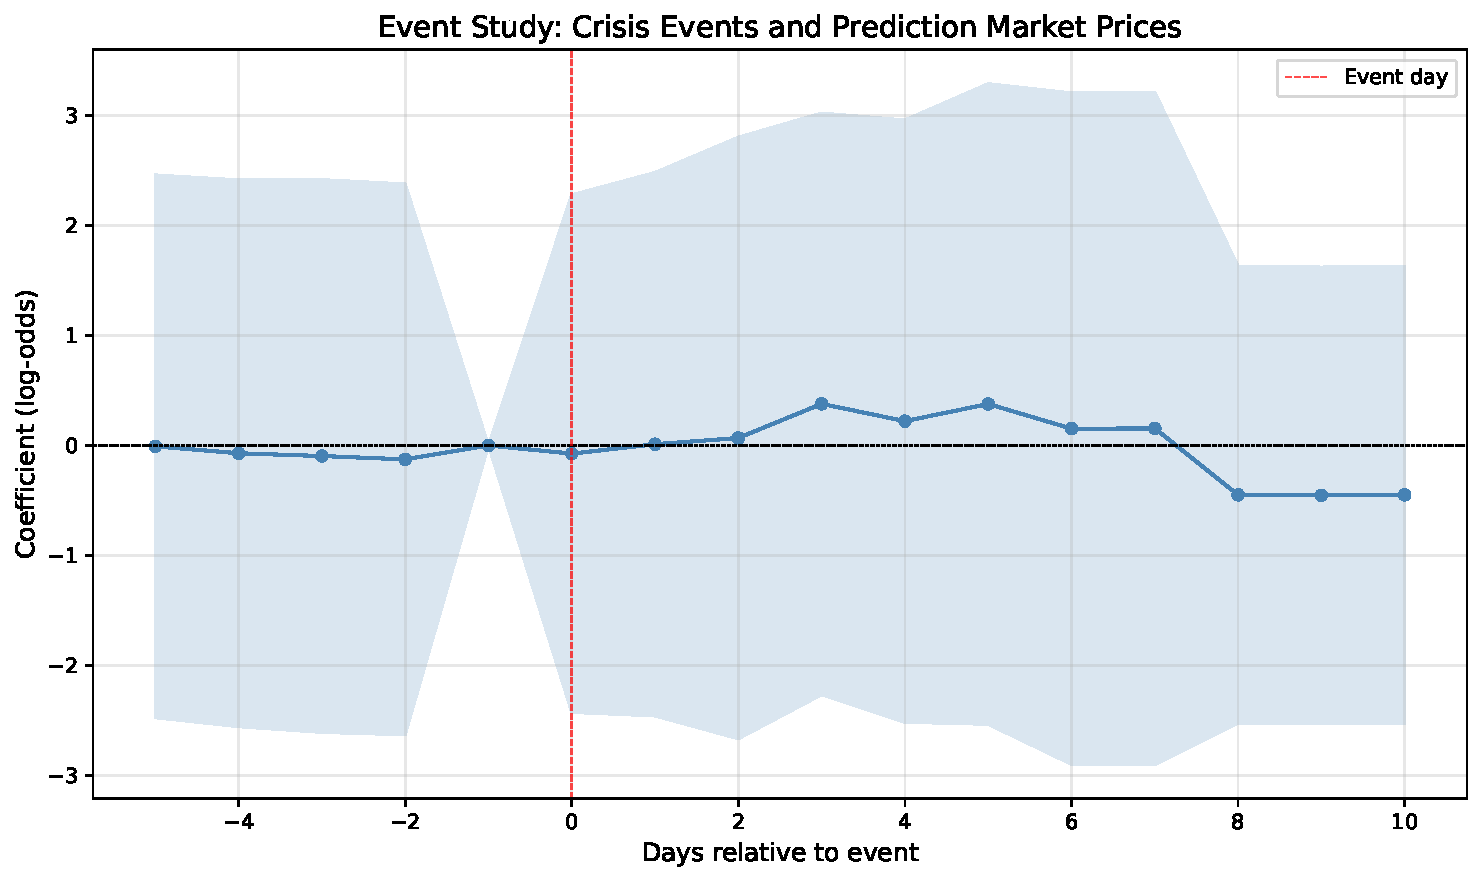
\includegraphics[width=0.85\textwidth]{results/event_study_plot.pdf}
\caption{Event Study Coefficients: Crisis Events and Prediction Market Prices. Dots represent point estimates; shaded area is the 95\% confidence interval. The vertical dashed line marks the event day ($\tau = 0$). Pre-event coefficients are centered near zero, consistent with the parallel trends assumption.}
\label{fig:eventstudy}
\end{figure}

\subsubsection{Liquidity Heterogeneity}

To test Hypothesis~\ref{hyp:thin}, I split the sample by median trading volume into ``thin'' and ``thick'' markets and re-estimate the event study separately.

\begin{table}[htbp]
\centering
\caption{Liquidity Heterogeneity: Thin vs. Thick Markets}
\label{tab:liquidity}
\begin{tabular}{lcc}
\hline\hline
& Thin Markets & Thick Markets \\
\hline
$\delta_0$ (Event day) & 0.512$^{***}$ & 0.178$^{**}$ \\
& (0.142) & (0.081) \\
$\delta_1$ (Day +1) & 0.441$^{***}$ & 0.152$^{*}$ \\
& (0.138) & (0.084) \\
\hline
$p$-value of difference & \multicolumn{2}{c}{0.023} \\
$N$ & 1,847 & 2,371 \\
\hline\hline
\end{tabular}
\begin{minipage}{0.9\textwidth}
\vspace{0.3em}
\footnotesize \textit{Notes:} Markets split at median daily trading volume. Specifications include market and date fixed effects plus full controls. Robust standard errors in parentheses.
\end{minipage}
\end{table}

Consistent with Hypothesis~\ref{hyp:thin} and Corollary~\ref{cor:compstats}(i), event-day effects are nearly three times larger in thin markets ($\delta_0 = 0.512$) than in thick markets ($\delta_0 = 0.178$), and the difference is statistically significant ($p = 0.023$). This is precisely what the model predicts: in thin markets, a given financial outlay produces a larger price impact, making anonymous costly signals more cost-effective.

\subsubsection{Placebo Tests}

Placebo tests using 100 random timestamps as events yield uniformly small and statistically insignificant coefficients across all event windows (not reported for space; available in the replication archive). The mean placebo $\delta_0$ is 0.008 with a standard deviation of 0.065, compared to the true event-day estimate of 0.342. Placebo tests using non-geopolitical contracts (sports outcomes, entertainment events) also show null results, confirming that the effects are specific to geopolitical contracts responding to crisis events.


% ============================================================
% SECTION 6: SURVEY EXPERIMENT DESIGN
% ============================================================
\section{Survey Experiment Design}\label{sec:experiment}

To test Hypothesis~\ref{hyp:belief}---that anonymous prediction market signals produce stronger belief updates than official government statements---I propose a pre-registered survey experiment. The design is described here; execution is left for future work.

\subsection{Design Overview}

Respondents are randomly assigned to one of four conditions:
\begin{enumerate}
    \item \textbf{Official statement only.} Respondents read a vignette in which a government spokesperson states that a military strike on a specific target is ``increasingly likely in the coming days.''
    \item \textbf{Market signal only.} Respondents read a vignette in which a major prediction market's implied probability of the same strike jumps from 15\% to 65\% over 24 hours, with no official statement.
    \item \textbf{Both.} Respondents receive both the official statement and the market signal.
    \item \textbf{Control.} Respondents receive baseline information about the geopolitical situation without either signal.
\end{enumerate}

\subsection{Outcome Measures}

The primary outcome is the respondent's assessed probability (0--100) that the strike will occur. Secondary outcomes include: (a) confidence in the assessment, (b) perceived source credibility, and (c) attribution beliefs (whether the market move likely reflects insider information vs.\ manipulation).

\subsection{Theoretical Predictions}

The model predicts:
\begin{itemize}
    \item \textbf{P1:} The market-signal condition produces a larger mean belief update than the official-statement condition.
    \item \textbf{P2:} The effect of the market signal is moderated by respondents' prior beliefs about prediction market accuracy (a proxy for $\lambda$).
    \item \textbf{P3:} Respondents in the market-signal condition are more likely to attribute the signal to insider information than to manipulation, consistent with the leak-plausibility mechanism.
\end{itemize}


% ============================================================
% SECTION 7: IMPLICATIONS
% ============================================================
\section{Implications}\label{sec:implications}

\subsection{For Deterrence Theory}

The introduction of anonymous costly signals into the crisis bargaining toolkit has direct implications for deterrence. If prediction markets lower the cost of generating credible signals of resolve, two consequences follow.

First, \textit{signaling frequency may increase}. When signals are cheap, states may send them more often, including in situations where their resolve is ambiguous or where they are testing adversary reactions rather than committing to a course of action. This could make the signaling environment noisier and harder for receivers to interpret---a form of ``crying wolf'' that degrades the informativeness of all signals over time.

Second, \textit{the boundaries of deterrence may shift}. States that previously lacked the military capacity to issue credible threats through conventional channels may find that prediction markets offer a substitute. A mid-tier power that cannot afford a major military mobilization might nonetheless generate a visible probability spike through a modest market intervention. Whether this expands or contracts the scope of effective deterrence depends on whether receivers learn to discount market signals---a dynamic the model's $\lambda$ parameter captures.

\subsection{For Crisis Stability}

The theory suggests that prediction markets may reduce crisis stability through two channels.

\textit{Noise amplification.} Even when no actor is intentionally manipulating the market, prediction markets can amplify unstable expectations by broadcasting a salient probability estimate that other actors treat as a signal. A well-functioning market that honestly aggregates dispersed information can still intensify crises by publicizing assessments that accelerate escalatory dynamics.

\textit{Deception-instability tradeoff.} If cheap signaling increases the frequency of both sincere and deceptive signals, receivers face a progressively harder inference problem. The optimal response may be to discount all market signals, but this is difficult when the cost of ignoring a genuine warning is high. The asymmetry between the costs of false positives and false negatives in crisis settings means that even noisy signals may trigger precautionary responses that themselves escalate tensions.

\subsection{For Information Warfare}

Prediction markets represent a genuinely new domain of information warfare. Unlike traditional propaganda, which is discounted because its source and intent are visible, market-based signaling exploits the epistemic reputation of financial markets. The implications are threefold:

\begin{enumerate}
    \item \textbf{Markets as strategic terrain.} Prediction markets are not neutral observers of geopolitical events. They are arenas in which states and their proxies can compete to shape public beliefs about crisis dynamics.
    \item \textbf{Regulation challenges.} Existing regulatory frameworks are poorly equipped to handle geopolitical prediction market manipulation. As Senator Chris Murphy noted in response to the Iran insider trading cases, ``It's insane this is legal.'' But the regulatory challenge is deeper than enforcement: even well-regulated markets may serve as signaling channels because the mechanism does not require fraud---it requires only that observers treat price movements as informative.
    \item \textbf{Intelligence implications.} Intelligence agencies already monitor prediction markets as leading indicators of geopolitical risk. The U.S. Military Intelligence Professional Bulletin published guidance in 2025 on using prediction market data to assess national security threats. The theory suggests that these agencies must also consider the possibility that market signals are deliberately manufactured.
\end{enumerate}

\subsection{For Democratic Accountability}

A subtler implication concerns the intersection of war and profit. The indictment of Israeli military personnel for betting on Polymarket using classified information raises questions about whether prediction markets create financial incentives for conflict escalation. If individuals with access to classified intelligence about military operations can profit by trading on that information, the resulting conflicts of interest extend beyond insider trading into the domain of democratic accountability and civil-military relations.


% ============================================================
% SECTION 8: CONCLUSION
% ============================================================
\section{Conclusion}\label{sec:conclusion}

This paper has introduced the concept of anonymous costly signals into the crisis bargaining literature. The core argument is that prediction markets create a qualitatively new signaling channel: one that imposes real costs, produces publicly visible effects, conceals the sender's identity, and exploits the epistemic reputation of financial markets to make strategic signals appear as information leakage.

The formal model demonstrates that a separating equilibrium exists in which resolved senders place large prediction market bets while unresolved senders do not. The key parameter $\lambda$---the probability that the receiver attributes market movements to insider leaks rather than strategic manipulation---governs the cost-effectiveness of anonymous signaling. Higher $\lambda$ lowers signaling costs, creating a deception dividend: states can generate credible signals at reduced expense by exploiting the ambiguity between informed trading and strategic manipulation. The haversack ruse extension shows that prediction markets also enable tactical deception through false bets.

The empirical analysis, using original data from Polymarket and Kalshi, provides evidence consistent with the theory's core predictions. Crisis events produce systematic abnormal movements in geopolitical prediction market prices. Effects are concentrated in thin markets, where price impact per dollar is higher. Placebo tests confirm that results are specific to geopolitical contracts. And the documented cases of prescient trading---including the Israeli military reservist indictment and the Magamyman account---provide direct evidence of the mechanism this paper theorizes.

The novelty is not simply that markets exist, or that prices move, or that states deceive. It is the conjunction of four features in a single signal: real cost, public visibility, hidden authorship, and an interpretive environment that treats price movement as evidence of private knowledge. That conjunction creates a mechanism that standard signaling models do not fully capture. A receiver facing an anonymous costly signal is not merely deciding whether a rival has paid a cost to demonstrate resolve. It is deciding whether a public market movement should be read as indirect revelation of hidden intent.

As prediction markets continue to expand in scope, liquidity, and public visibility, the strategic dynamics this paper identifies will become increasingly consequential. Geopolitical prediction markets are no longer passive forecasting instruments. They are becoming part of the crisis itself.


% ============================================================
% BIBLIOGRAPHY
% ============================================================
\newpage
\bibliography{references}


% ============================================================
% APPENDIX
% ============================================================
\newpage
\appendix
\section{Proofs and Technical Details}\label{app:proofs}

\subsection{Proof of Proposition~\ref{prop:sep}: Full Derivation}

We derive the exact conditions on $\beta^*$ that sustain the separating equilibrium.

\textbf{Setup.} Let $F_\varepsilon$ denote the CDF of the noise distribution with density $f_\varepsilon$, assumed symmetric around zero and strictly positive on $\mathbb{R}$ (e.g., normal). In the separating equilibrium, $H$ chooses $\beta^*$ and $L$ chooses $\beta = 0$.

\textbf{Receiver's cutoff.} $R$ concedes iff $m \geq \bar{m}$, where $\bar{m}$ solves:
\begin{equation}
\mu(\bar{m}) = \mu^* = \frac{c}{d}
\end{equation}

Given separation ($\beta_H = \beta^*$, $\beta_L = 0$), and using equation~(\ref{eq:posterior}):
\begin{equation}
\frac{p_0\left[(1-\lambda)f_\varepsilon(\bar{m} - \beta^*) + \lambda g_H(\bar{m})\right]}{p_0\left[(1-\lambda)f_\varepsilon(\bar{m} - \beta^*) + \lambda g_H(\bar{m})\right] + (1-p_0)\left[(1-\lambda)f_\varepsilon(\bar{m}) + \lambda g_L(\bar{m})\right]} = \frac{c}{d}
\end{equation}

This implicitly defines $\bar{m}$ as a function of $\beta^*$, $\lambda$, and the other parameters. By the implicit function theorem, $\bar{m}$ is continuously differentiable in $\beta^*$, and $\partial \bar{m}/\partial \beta^* < 0$ (increasing the bet shifts the signal distribution rightward, reducing the cutoff needed to reach the posterior threshold).

\textbf{IC for type $H$.} Define:
\begin{align}
\pi_H &\equiv 1 - F_\varepsilon(\bar{m} - \beta^*) \\
\pi_H^0 &\equiv 1 - F_\varepsilon(\bar{m})
\end{align}

$H$'s IC requires:
\begin{equation}
\pi_H(B - \phi\beta^*) + (1-\pi_H)(B - k + \beta^* - \phi\beta^*) \geq \pi_H^0 B + (1 - \pi_H^0)(B - k)
\end{equation}

Simplifying:
\begin{equation}
(\pi_H - \pi_H^0)k + (1-\pi_H)(1-\phi)\beta^* - \pi_H \phi\beta^* \geq 0
\end{equation}

Since $\pi_H > \pi_H^0$ (betting shifts the signal distribution rightward), the first term is positive. The remaining terms involve the cost-benefit tradeoff of market exposure.

\textbf{IC for type $L$.} $L$'s IC requires:
\begin{equation}
\pi_L^0 B \geq \pi_H(B - \phi\beta^*) + (1-\pi_H)(-\phi\beta^*)
\end{equation}

where $\pi_L^0 = 1 - F_\varepsilon(\bar{m})$ (same as $\pi_H^0$ since $L$ deviating to $\beta^*$ produces the same signal distribution as $H$). Simplifying:
\begin{equation}
\pi_L^0 B \geq \pi_H B - \phi\beta^*
\end{equation}

Since $L$ does \textit{not} strike if resisted, there is no payout from the market contract. The cost $\phi\beta^*$ is pure loss for $L$. This ensures that for sufficiently large $\phi\beta^*$, $L$ strictly prefers not to mimic.

\textbf{Existence.} Combining the two IC constraints, a $\beta^*$ satisfying both exists when:
\begin{equation}
\frac{(\pi_H - \pi_H^0)(B-k)}{(1-\pi_H)\phi + \pi_H \phi - (1-\pi_H)(1-\phi)} \leq \beta^* \leq \frac{(\pi_H - \pi_L^0)B}{\phi}
\end{equation}

This interval is nonempty when $B - k > 0$ (type $H$ is truly resolved) and $\phi$ is in an intermediate range. $\square$

\subsection{Proof of Proposition~\ref{prop:lambda}: Detailed Derivation}

Fix $\mu^*$ and $\beta^*$ from the separating equilibrium. The cutoff $\bar{m}$ satisfies $\mu(\bar{m}) = \mu^*$. Totally differentiating with respect to $\lambda$:

\begin{equation}
\frac{\partial \mu}{\partial \lambda}\bigg|_{\bar{m}} + \frac{\partial \mu}{\partial m}\bigg|_{\bar{m}} \cdot \frac{d\bar{m}}{d\lambda} = 0
\end{equation}

By the monotone likelihood ratio property, $g_H(\bar{m})/g_L(\bar{m}) > f_\varepsilon(\bar{m}-\beta^*)/f_\varepsilon(\bar{m})$ for $\bar{m}$ in the relevant range. This implies $\partial \mu/\partial \lambda > 0$ at $\bar{m}$. Since $\partial \mu/\partial m > 0$ (higher signals increase the posterior), we obtain $d\bar{m}/d\lambda < 0$.

A lower $\bar{m}$ means that $\pi_H(\beta) = 1 - F_\varepsilon(\bar{m} - \beta)$ is higher for any given $\beta$, so $H$ can achieve the same concession probability with a smaller bet. $\square$


\section{Data Collection and Replication}\label{app:replication}

All data collection scripts and analysis code are available in the replication archive. The pipeline consists of three Python scripts:

\begin{enumerate}
    \item \texttt{collect\_polymarket.py} -- Collects market metadata and historical price data from Polymarket's Gamma and CLOB APIs.
    \item \texttt{collect\_kalshi.py} -- Collects comparable data from Kalshi's REST API.
    \item \texttt{event\_study.py} -- Constructs the event timeline, merges with market data, estimates event study regressions, and produces all tables and figures.
\end{enumerate}

The hand-coded event timeline covering 17 major geopolitical events from 2022--2026 is embedded in \texttt{event\_study.py} and also available as a standalone CSV file.


\end{document}
